
%-----------------------------------------------------------------------------
%
%               Template for LaTeX Class/Style File
%
% Name:         sigplanconf-template.tex
% Purpose:      A template for sigplanconf.cls, which is a LaTeX 2e class
%               file for SIGPLAN conference proceedings.
%
% Author:       Paul C. Anagnostopoulos
%               Windfall Software
%               978 371-2316
%               paul@windfall.com
%
% Created:      15 February 2005
%
%-----------------------------------------------------------------------------
\documentclass{sigplanconf}
%\documentclass[letterpaper,twocolumn,10pt]{article}



\usepackage{usenix,epsfig,endnotes,url,color,subfigure}
\usepackage{array}
\usepackage{multirow}
\usepackage{xspace}
\usepackage{verbatim}
\usepackage{hyperref}
\usepackage[compact]{titlesec}
\usepackage{wrapfig}



\usepackage[english]{babel}

\usepackage{amsmath}
 \usepackage[ruled]{algorithm2e}


 % Add navigation window to pdf
\usepackage{hyperref}
\hypersetup{pdftex,colorlinks=true,allcolors=blue}
\usepackage{hypcap}


%%%%%%%%%%%%%%%%%%%%%%%%%%%%%%%%%%%%%%%%%%%%%%%%%%%%%%%%%%%%%%%%%%%%%%
%% mac.tex
%%
%% Umut A. Acar
%% Macros for adaptive computation paper.
%%%%%%%%%%%%%%%%%%%%%%%%%%%%%%%%%%%%%%%%%%%%%%%%%%%%%%%%%%%%%%%%%%%%%%

\newcommand{\readarrow}{\ensuremath{\Longrightarrow}}
\newcommand{\currenttime}{\ttt{currentTime}\xspace}
\newcommand{\tags}[1]{\ensuremath{\mathsf{tags}(#1)}}
\newcommand{\weight}[1]{\ensuremath{\mathsf{weight}(#1)}}
\newcommand{\dist}[2]{\ensuremath{\delta(#1,#2)}}


\newcommand{\cutspace}{\vspace{-4mm}}

\newcommand{\bomb}[1]{\fbox{\mbox{\emph{\bf {#1}}}}}

\newcommand{\myparagraph}[1]{\smallskip \noindent{\bf {#1}.}}
% formatting stuff
\newcommand{\codecolsep}{1ex}



\newcommand{\rlabel}[1]{\hspace*{-1mm}\mbox{\small{\bf ({#1})}}}

\newcommand{\tablerow}{\\[5ex]}
\newcommand{\tableroww}{\\[7ex]}
\newcommand{\tableline}{
\vspace*{2ex}\\
\hline\\
\vspace*{2ex}}

% Don't care
\newcommand{\dontcare}{\_
}

%% filter and quicksort stuff
\newcommand{\ncf}[2]{C^{fil}_{\ensuremath{{#1},{#2}}}}
\newcommand{\ncq}[1]{C^{qsort}_{\ensuremath{#1}}}
\newcommand{\nuf}[3]{P^{fil}_{#1,(\ensuremath{{#2},{#3}})}}
\newcommand{\nuq}[2]{P^{qsort}_{(\ensuremath{{#1},{#2}})}}

%% shorthands
\newcommand{\ddg}{{\sc ddg}}
\newcommand{\ncpa}{change-propagation algorithm}
\newcommand{\adg}{{\sc adg}}
\newcommand{\nwrite}{\texttt{write}}
\newcommand{\nread}{\texttt{read}}
\newcommand{\nmodr}{\texttt{mod}}
\newcommand{\ttt}[1]{\texttt{#1}}
\newcommand{\nmodl}{\texttt{modl}}
\newcommand{\nnil}{\ttt{NIL}}
\newcommand{\ncons}[2]{\ttt{CONS({\ensuremath{#1},\ensuremath{#2}})}}
\newcommand{\nfilter}{\texttt{filter}}
\newcommand{\nfilterp}{\texttt{filter'}}
\newcommand{\naqsort}{\texttt{qsort'}}
\newcommand{\nqsort}{\texttt{qsort}}
\newcommand{\nqsortp}{\texttt{qsort'}}
\newcommand{\nnewMod}{\texttt{newMod}}
\newcommand{\nchange}{\texttt{change}}
\newcommand{\npropagate}{\texttt{propagate}}
\newcommand{\ndest}{\texttt{d}}
\newcommand{\ninit}{\texttt{init}}



%% Comment sth out.
\newcommand{\out}[1] {}
\newcommand{\sthat}{\ensuremath{~|~}}

%% definitions
\newcommand{\defi}[1]{{\bfseries\itshape #1}}


% Code listings.
\newcounter{codeLineCntr}
\newcommand{\codeLine}
 {\refstepcounter{codeLineCntr}{\thecodeLineCntr}}
\newcommand{\codeLineL}[1]
 {\refstepcounter{codeLineCntr}\label{#1}{\thecodeLineCntr}}
\newcommand{\codeLineNN}{} %% NN = No-Number (and no change to counter)

\newenvironment{codeListing}
 {\setcounter{codeLineCntr}{0}
%  \fontsize{10}{12}
 % the first one is width the second is height
 \fontsize{9}{11}
  \fontsize{8}{8}
  \vspace{-.1in}
  \ttfamily\begin{tabbing}}
  {\end{tabbing}
   \vspace{-.1in}}

\newenvironment{codeListing8}
 {\setcounter{codeLineCntr}{0}
%  \fontsize{8}{10}
  \fontsize{8}{8}
  \vspace{-.1in}
  \ttfamily
  \begin{tabbing}}
 {\end{tabbing}
 \vspace{-.1in}
}

\newenvironment{codeListing8h}
 {\setcounter{codeLineCntr}{0}
  \fontsize{8.5}{10.5}
  \vspace{-.1in}
  \ttfamily
  \begin{tabbing}}
 {\end{tabbing}
 \vspace{-.1in}
}


\newenvironment{codeListing9}
 {\setcounter{codeLineCntr}{0}
  \fontsize{9}{11}
  \vspace{-.1in}
  \ttfamily
  \begin{tabbing}}
 {\end{tabbing}
 \vspace{-.1in}
}

\newenvironment{codeListing10}
 {\setcounter{codeLineCntr}{0}
  \fontsize{10}{12}
  \vspace{-.1in}
  \ttfamily
  \begin{tabbing}}
 {\end{tabbing}
 \vspace{-.1in}
}


\newenvironment{codeListingNormal}
 {\setcounter{codeLineCntr}{0}
  \vspace{-.1in}
  \ttfamily
  \begin{tabbing}}
 {\end{tabbing}
 \vspace{-.1in}
}

\newcommand{\codeFrame}[1]
{\begin{center}\fbox{\parbox[t]{\columnwidth}{#1}}\end{center}
% \vspace*{-.15in}
}

\newcommand{\halfBox}[1]
{\begin{center}\fbox{\parbox[t]{\columnwidth}{#1}}\end{center}
% \vspace*{-.15in}
}

\newcommand{\fullBox}[1]
{\begin{center}\fbox{\parbox[t]{\textwidth}{#1}}\end{center}
% \vspace*{-.15in}
}

%%Note this is redefined in local-mac.tex for each paper.
\newcommand{\fixedCodeFrame}[1]
{
\begin{center}
\fbox{
\parbox[t]{0.9\columnwidth}{
#1
}
}\end{center}
}

% Footnote commands.
\newcommand{\footnotenonumber}[1]{{\def\thempfn{}\footnotetext{#1}}}

% Margin notes - use \notesfalse to turn off notes.
\setlength{\marginparwidth}{0.6in}
\reversemarginpar
\newif\ifnotes
\notestrue
\newcommand{\longnote}[1]{
  \ifnotes
    {\medskip\noindent Note:\marginpar[\hfill$\Longrightarrow$]
      {$\Longleftarrow$}{#1}\medskip}
  \fi}
\newcommand{\note}[1]{
  \ifnotes
    {\marginpar{\raggedright{\tiny #1}}}
  \fi}
\newcommand{\notered}[1]{\ifnotes
    {\marginpar{\raggedright{\tiny
          {\sf\color{red} #1}}}}
    \fi}


% Stuff not wanted.
\newcommand{\punt}[1]{}

% Sectioning commands.
\newcommand{\subsec}[1]{\subsection{\boldmath #1 \unboldmath}}
\newcommand{\subheading}[1]{\subsubsection*{#1}}
\newcommand{\subsubheading}[1]{\paragraph*{#1}}

% Reference shorthands.
\newcommand{\spref}[1]{Modified-Store Property~\ref{sp:#1}}
\newcommand{\prefs}[2]{Properties~\ref{p:#1} and~\ref{p:#2}}
\newcommand{\pref}[1]{Property~\ref{p:#1}}


\newcommand{\partref}[1]{Part~\ref{part:#1}}
\newcommand{\chref}[1]{Chapter~\ref{ch:#1}}
\newcommand{\chreftwo}[2]{Chapters \ref{ch:#1} and~\ref{ch:#2}}
\newcommand{\chrefthree}[3]{Chapters \ref{ch:#1}, and~\ref{ch:#2}, and~\ref{ch:#3}}
\newcommand{\secref}[1]{Section~\ref{sec:#1}}
\newcommand{\subsecref}[1]{Subsection~\ref{subsec:#1}}
\newcommand{\secreftwo}[2]{Sections \ref{sec:#1} and~\ref{sec:#2}}
\newcommand{\secrefthree}[3]{Sections \ref{sec:#1},~\ref{sec:#2},~and~\ref{sec:#3}}
\newcommand{\appref}[1]{Appendix~\ref{app:#1}}
\newcommand{\figref}[1]{Figure~\ref{fig:#1}}
\newcommand{\figreftwo}[2]{Figures \ref{fig:#1} and~\ref{fig:#2}}
\newcommand{\figrefthree}[3]{Figures \ref{fig:#1}, \ref{fig:#2} and~\ref{fig:#3}}
\newcommand{\figreffour}[4]{Figures \ref{fig:#1},~\ref{fig:#2},~\ref{fig:#3}~and~\ref{fig:#4}}
\newcommand{\figpageref}[1]{page~\pageref{fig:#1}}
\newcommand{\tabref}[1]{Table~\ref{tab:#1}}
\newcommand{\tabreftwo}[2]{Tables~\ref{tab:#1} and~\ref{tab:#1}}

\newcommand{\stref}[1]{step~\ref{step:#1}}
\newcommand{\caseref}[1]{case~\ref{case:#1}}
\newcommand{\lineref}[1]{line~\ref{line:#1}}
\newcommand{\linereftwo}[2]{lines \ref{line:#1} and~\ref{line:#2}}
\newcommand{\linerefthree}[3]{lines \ref{line:#1},~\ref{line:#2},~and~\ref{line:#3}}
\newcommand{\linerefrange}[2]{lines \ref{line:#1} through~\ref{line:#2}}
\newcommand{\thmref}[1]{Theorem~\ref{thm:#1}}
\newcommand{\thmreftwo}[2]{Theorems \ref{thm:#1} and~\ref{thm:#2}}
\newcommand{\thmrefthree}[3]{Theorems \ref{thm:#1}, \ref{thm:#2} and~\ref{thm:#3}}
\newcommand{\thmpageref}[1]{page~\pageref{thm:#1}}
\newcommand{\lemref}[1]{Lemma~\ref{lem:#1}}
\newcommand{\lemreftwo}[2]{Lemmas \ref{lem:#1} and~\ref{lem:#2}}
\newcommand{\lemrefthree}[3]{Lemmas \ref{lem:#1},~\ref{lem:#2},~and~\ref{lem:#3}}
\newcommand{\lempageref}[1]{page~\pageref{lem:#1}}
\newcommand{\corref}[1]{Corollary~\ref{cor:#1}}
\newcommand{\defref}[1]{Definition~\ref{def:#1}}
\newcommand{\defreftwo}[2]{Definitions \ref{def:#1} and~\ref{def:#2}}
\newcommand{\defpageref}[1]{page~\pageref{def:#1}}
\renewcommand{\eqref}[1]{Equation~(\ref{eq:#1})}
\newcommand{\eqreftwo}[2]{Equations (\ref{eq:#1}) and~(\ref{eq:#2})}
\newcommand{\eqpageref}[1]{page~\pageref{eq:#1}}
\newcommand{\ineqref}[1]{Inequality~(\ref{ineq:#1})}
\newcommand{\ineqreftwo}[2]{Inequalities (\ref{ineq:#1}) and~(\ref{ineq:#2})}
\newcommand{\ineqpageref}[1]{page~\pageref{ineq:#1}}
\newcommand{\itemref}[1]{Item~\ref{item:#1}}
\newcommand{\itemreftwo}[2]{Item~\ref{item:#1} and~\ref{item:#2}}

% Useful shorthands.
\newcommand{\abs}[1]{\left| #1\right|}
\newcommand{\card}[1]{\left| #1\right|}
\newcommand{\norm}[1]{\left\| #1\right\|}
\newcommand{\floor}[1]{\left\lfloor #1 \right\rfloor}
\newcommand{\ceil}[1]{\left\lceil #1 \right\rceil}
  \renewcommand{\choose}[2]{{{#1}\atopwithdelims(){#2}}}
\newcommand{\ang}[1]{\langle#1\rangle}
\newcommand{\paren}[1]{\left(#1\right)}
\newcommand{\prob}[1]{\Pr\left\{ #1 \right\}}
\newcommand{\expect}[1]{\mathrm{E}\left[ #1 \right]}
\newcommand{\expectsq}[1]{\mathrm{E}^2\left[ #1 \right]}
\newcommand{\variance}[1]{\mathrm{Var}\left[ #1 \right]}
\newcommand{\twodots}{\mathinner{\ldotp\ldotp}}

% Standard number sets.
\newcommand{\reals}{{\mathrm{I}\!\mathrm{R}}}
\newcommand{\integers}{\mathbf{Z}}
\newcommand{\naturals}{{\mathrm{I}\!\mathrm{N}}}
\newcommand{\rationals}{\mathbf{Q}}
\newcommand{\complex}{\mathbf{C}}

% Special styles.
\newcommand{\proc}[1]{\ifmmode\mbox{\textsc{#1}}\else\textsc{#1}\fi}
\newcommand{\procdecl}[1]{
  \proc{#1}\vrule width0pt height0pt depth 7pt \relax}
  \newcommand{\func}[1]{\ifmmode\mathrm{#1}\else\textrm{#1}fi} %
%  Multiple cases.
\renewcommand{\cases}[1]{\left\{
  \begin{array}{ll}#1\end{array}\right.}
  \newcommand{\cif}[1]{\mbox{if $#1$}}

%% spacing hacks
\newcommand{\longpage}{\enlargethispage{\baselineskip}}
\newcommand{\shortpage}{\enlargethispage{-\baselineskip}}



%% Notes, todos, and remarks
\newcounter{remark}[section]

\newcommand{\myremark}[3]{
\refstepcounter{remark}
\[
\left\{
\sf
\parbox{\columnwidth}{
{\bf {#1}'s remark~\theremark:}
{#3}
}
\right\}
\]
%\marginpar{\bf {#2}.~\theremark}
}


% - - - - - - - - - - - - - - - - - - - - - - - - - - - - - - - - - - - - - - - - - - - -
% For amsthm package:

%\theoremstyle{plain}
%\newtheorem{thm}{Theorem}[section]
%% \newtheorem{lem}[thm]{Lemma}
%% \newtheorem{prop}[thm]{Proposition}
%% \newtheorem*{cor}{Corollary}

%% \theoremstyle{definition}
%% \newtheorem{defn}{Definition}[section]
%% \newtheorem{conj}{Conjecture}[section]
%% \newtheorem{falseconj}{False~Conjecture}[section]
%% \newtheorem{exmp}{Example}[section]

%% \theoremstyle{remark}
%% \newtheorem*{rem}{Remark}
%% %\newtheorem*{note}{Note}
%% \newtheorem{case}{Case}


\newcommand{\uremark}[1]{\myremark{Umut}{U}{#1}}
\newcommand{\ur}[1]{\uremark{#1}}
\newcommand{\rremark}[1]{\myremark{Ruy}{R}{#1}}
\newcommand{\mremark}[1]{\myremark{Matthew}{M}{#1}}
\newcommand{\todoremark}[1]{\myremark{TODO}{TODO}{#1}}
%\newcommand{\todo}[1]{\myremark{TODO}{TODO}{#1}}
\newcommand{\todo}[1]{{\bf{[TODO:{#1}]}}}

%%

%%
%% Functions
\newcommand{\timeOfTask}[1]{\ensuremath{t_T {#1} }}
\newcommand{\timeRead}[1]{\ensuremath{t_R {#1} }}
\newcommand{\timeWrite}[1]{\ensuremath{t_W {#1} }}


%% sets
\newcommand{\setFresh}{\mathcal{F}}
\newcommand{\setReused}{\mathcal{R}}


%% times
\newcommand{\timeHash}{\ensuremath{t_h}\xspace}
\newcommand{\timeMessage}{\ensuremath{t_m}\xspace}
\newcommand{\timeMemo}{\ensuremath{t_{memo}}\xspace}
\newcommand{\ninput}{\ensuremath{n_i}\xspace}
\newcommand{\noutput}{\ensuremath{n_O}\xspace}
\newcommand{\nmap}{\ensuremath{N_M}\xspace}
\newcommand{\nred}{\ensuremath{N_R}\xspace}
\newcommand{\ncon}{\ensuremath{N_C}\xspace}

\newcommand{\nkeysetmap}{\ensuremath{n_{mk}}}
\newcommand{\nkeyvaluemap}{\ensuremath{n_{m}}}
\newcommand{\nconAppend}{\ensuremath{H_{CA}}\xspace}
\newcommand{\nconFix}{\ensuremath{H_{CF}}\xspace}
\newcommand{\nconVariable}{\ensuremath{H_{CV}}\xspace}

%% numbers
\newcommand{\numberTasks}{\ensuremath{n_t}}
\newcommand{\inputSize}{\ensuremath{s_i}}
\newcommand{\avgChunkSize}{\ensuremath{s_c}}
\newcommand{\keyset}{\ensuremath{K}}


%% sizes
\newcommand{\sizeReducers}{\ensuremath{m_r}}


\newcommand{\myfontsize}{\fontsize{8}{9}\selectfont}

\newcommand{\graph}{{Concurrent Execution Graph (CEG)}\xspace}

\newcommand{\projecttitle}{{\tt Inspector}\xspace}
\newcommand{\pthreads}{{\tt pthreads}\xspace}
\newcommand{\dthreads}{{\tt Dthreads}\xspace}
\newcommand{\intelpt}{{Intel\textsuperscript{\textregistered} PT}\xspace}

%\newcommand{\todo}[1]{{\frameit{ToDo}{#1}}}
\newcommand{\obs}[1]{{\frameit{Obs}{#1}}}
% \usepackage{amsthm}
\newtheorem{lemma}{Lemma}
\newtheorem{theorem}{Theorem}

\pagenumbering{arabic}


\usepackage{mathpazo} % math & rm
\linespread{1.03}        % Palatino needs more leading (space between lines)
%\usepackage{inconsolata}
%\usepackage{zi4}
%\renewcommand{\ttdefault}{txtt}
\normalfont
\usepackage[T1]{fontenc}


\begin{document}
\title{Inspector: An Execution Synthesis Library for Multithreaded Programs}

\authorinfo{Name1}
           {Affiliation1}
           {Email1}
\authorinfo{Name2\and Name3}
           {Affiliation2/3}
           {Email2/3}

%\author{
%\parbox{1.5in}{
%\centerline{J\"{o}rg Thalheim}
%\centerline{TU Dresden}
%}
%\and
%\parbox{1.5in}{
%\centerline{Pramod Bhatotia}
%\centerline{TU Dresden}
%}
%\and
%\parbox{1.5in}{
%\centerline{Christof Fetzer}
%\centerline{TU Dresden}
%}
%}


\maketitle
%\thispagestyle{empty}
%\pagestyle{empty}
\begin{abstract}
Data provenance strives for {\em explaining} how the computation was performed, by recording a ``trace" of the execution. The provenance trace is useful for a wide-range of workflows in improving the dependability, security, and efficiency of software systems. 

In this paper, we present \projecttitle\footnote{For the double-blind review process, we have changed the name to \projecttitle.}, a {\tt POSIX}-compliant data provenance library for shared-memory multithreaded programs. The \projecttitle library is completely transparent and easy to use: it can be used as a replacement for the \pthreads library by a simple exchange of libraries linked, without even recompiling the code.  


To achieve this result,  we present a parallel provenance algorithm that records control, data, and schedule dependencies using  a {\em Concurrent Provenance Graph} (CPG).  We implemented our algorithm to operate at the compiled binary code
level by leveraging a combination of OS-specific mechanisms, and recently released \intelpt ISA extensions as part of the Broadwell and Skylake microarchitectures.  Our
evaluation on a multicore platform using applications from multithreaded benchmarks suites (PARSEC
and Phoenix) shows reasonable overheads for recording the data provenance trace. 

Furthermore, we briefly describe three on-going case-studies where the generic provenance interface exported by \projecttitle is being used to improve the dependability, security, and efficiency of software systems. \projecttitle is an active open-source project and the tool is publicly available to the research community for use in other workflows. 

\end{abstract}



\section{Introduction}
\label{sec:introduction}

Data provenance provides an explicit intermediate program representation recording control and data dependencies for a program execution~\cite{pdg-pingali}.  proved to be one of the important abstractions in program analysis as the concept is used for a wide range of workflows; including, program debugging, compiler optimizations, data provenance, incremental computation, program slicing, dynamic flow information control and tracking,  etc.


\if 0
Multithreaded programs are notoriously difficult to debug. This difficulty arises from the fact that multithreaded programs are inherently non-deterministic. Consequently, threads accessing the shared-memory region with different inter-leavings may lead to undesirable concurrency bugs, like program crash or data corruption. 


Currently, debugging techniques rely on examining memory state during the program execution or by analyzing core dumps after the program crashes. These techniques mainly target ``what" is the state of the program without revealing much about ``why" is it the state of the program like that. We can aid the developers to better understand the failed execution by augmenting the existing debugging techniques with the lineage information of the memory state or ``why"-provenance or simply data-provenance.

 \fi
%Many existing systems provide support for data provenance; however,
%most target sequential programs (detailed in $\S$~\ref{sec:related}),
%while others that do support parallelism require a new language with a restrictive programming model. Furthermore, the existing  provenance systems for parallel programs rely on manual annotations using a new type system. Thereby, limiting their wide-spread adoption.



In this paper, we propose an OS-based approach to data provenance for multithreaded programs. More specifically, we have two main design goals: (1) To support unmodified shared-memory multithreaded programs with the full range of synchronization primitives in the {\tt POSIX} API; (2) To achieve low overheads by designing the underlying provenance algorithm to be  {\em parallel} as well that does not limit the available application parallelism.


To achieve these goals, we present \projecttitle, a threading library for data provenance. To run a program using \projecttitle,  the user just needs to preload the \projecttitle library  by using the environment variable {\tt LD\_PRELOAD} or {\tt -rdynamic} flag, and then, run the program as usual. Thus, enabling existing binaries to benefit from our approach. 


Our approach is based on recording the data and control dependencies in a computation by constructing a Concurrent Provenance Graph (CPG). The CPG tracks the input data to a program, all sub-computations (a sub-computation is a unit of the computation), the data flow between sub-computations, and intra- and inter-thread control flow of the multithreaded execution.


Overall, this paper makes the following contributions:
\begin{itemize}

\item We present a parallel algorithm for data provenance for multithreaded programs that records intra- and inter-thread control and data dependencies using a Concurrent Provenance Graph (CPG) (\secref{algorithms}).

\item We implemented our algorithm as a dynamically linkable shared library, which we call \projecttitle, leveraging MMU-assisted memory tracking, process-level isolation, and recently released \intelpt ISA extensions.  The \projecttitle library can be loaded and linked at run-time as a replacement to the \pthreads library, without any recompilation  of the application code (\secref{implementation}).

\item  We  empirically demonstrate  the effectiveness of \projecttitle by applying it to applications of standard multithreaded benchmark suites (PARSEC~\cite{parsec} and Phoneix~\cite{phoenix}). Our experiments show that \projecttitle~incurs reasonable overhead for a majority of applications (\secref{evaluation}). 

\end{itemize}

\projecttitle is an active open-source project, and the library is publicly available to the research community. We believe that the CPG abstraction exported by \projecttitle can be used to support of a wide-range of workflows in dependability and security, as discussed in %$$~\ref{sec:discussion}.

\section{Overview}
\label{sec:overview}
%
%Our approach targets a shared-memory multithreaded environment, in which threads parallelize computation and take 
%advantage of shared portions of the address space to efficiently communicate with each other. Apart from performing reads 
%and writes to the shared memory, threads also employ different types of synchronization mechanisms to 
%co-ordinate their progress, thereby ensuring correct semantics. 

%We base our design on {\tt POSIX} threads, commonly referred to as
%{\tt pthreads}, which is a widely used threading library for shared-memory
%multithreading with a rich set of synchronization primitives.  This
%choice has several advantages, namely that the {\tt POSIX} interface
%is standardized across different architectures and operating systems. Furthermore, {\tt pthreads} is used as the underlying threading
%library for many higher level abstractions for parallel programming
%(e.g., {\tt OpenMP}). Therefore, our design choice benefits a lot of existing applications.

We base our design on {\tt POSIX} threads, commonly referred to as
{\tt pthreads}, a widely used threading library for shared-memory
multithreading with a rich set of synchronization primitives.  


\myparagraph{Basic approach} At a high level, we record data provenance for a multithreaded execution by constructing a {\em Concurrent Provenance Graph (or CPG)}. Informally,  the CPG records three types of dependencies; namely, control, data, and schedule dependencies for the multithreaded execution. To record these dependencies, we divide thread execution into sub-computations. We record the execution trace to construct the CPG that tracks the {\em data flow} between the sub-computations, {\em control flow} for each thread execution, and threads interleaving or {\em schedule dependency}  in the multithreaded execution.

More specifically, the Concurrent Provenance Graph (or CPG) records a partial order $O = (N, \rightarrow$) among sub-computations with the following property: given a sub-computation $n$ (where $n \in N $)  and the subset of sub-computations $M$ that precede it according to $\rightarrow$, i.e., $M = \{M \subset N \mid \forall m \in M,$ $m \rightarrow n\}$, if the writes made by $m$ becomes visible to $n$ then the partial order $\rightarrow$ captures this possible data flow between sub-computations.

%We next use a simple example to explain the high-level approach (shown in Figure~\ref{fig:simple-example}). 



\myparagraph{Example} Using a simple example (shown in Figure~\ref{fig:simple-example}), we next explain how do we record these dependencies for a shared-memory multithreaded program. The example considers a multithreaded execution with two threads ($T_1$ and $T_2$) modifying two shared variables ($x$ and $y$) using a lock. In the example, we assume that a thread execution is divided into sub-computations at the boundaries of synchronization primitives, such as {\tt lock()/unlock()}. (We explain the reason behind this design choice in $\S$\ref{sec:model}.) We identify these sub-computations as $T_1.a$ and $T_1.b$ for thread $T_1$, and $T_2.a$ for thread $T_2$.   To understand the dependencies that need to be recorded for the required partial order ($\rightarrow$), we showcase three cases for recording the control, schedule, and data dependencies.

The first dependency that we need to record is the {\em control flow} execution of each thread. In particular, we need to record the intra-thread execution order of sub-computations. For example, sub-computation $T_1.b$ follows $T_1.a$, and therefore, the control flow dependency records this partial order as $T_1.a \rightarrow T_1.b$. Additionally, we need to record the control flow path taken within a sub-computation. For example, sub-computation  $T_1.a$ has a conditional branch ({\tt if/else}) based on the value of {\tt flag}. We supplement the control flow dependency with all control paths taken by a thread within each sub-computation; i.e.,  all branches taken at run-time.

Secondly, we need to record the inter-thread {\em schedule} dependencies. The sub-computations can be interleaved in different order across executions because of the non-deterministic thread scheduling by the underlying OS. For instance, when threads acquiring the lock in the reverse order where thread $T_1.b$ gets acquire the lock before $T_2.a$. In this case, the final value of $y$ is affected based on this new ordering. Therefore, we also need to record the schedule dependencies between sub-computations as part of the partial order. We record these schedule dependencies by tracking interleaving of sub-computations by recording the thread schedule (For example, $T_1.a   \rightarrow   T_2.a \rightarrow T_1.b $).

Lastly,   we need to record {\em data dependencies} between sub-computations as a part of the partial order. For that we track read and write sets for each sub-computation, i.e., the set of memory locations read or written by the sub-computation, respectively. The data dependencies are recorded implicitly using read and write-sets, and the partial order recorded using the control and schedule dependencies: if we know what data is read and written by each sub-computation, we can determine whether a data dependency exists by following the partial order, i.e. if a sub-computation is {\em transitively} reading the data that was modified by a sub-computation that precedes it in the partial order $\rightarrow$ then there exists a read-after-write data dependency. 

%, i.e., if a sub-computation is reading data that was modified by another sub-computation, which might have required recomputation in the incremental run.



%consider a case of the input change where the value of variable $y$ is changed during an execution. Assuming that thread $T_1$ gets to acquire the lock before thread $T_2$, the writes made by sub-computation $T_1.a$ will affect the read made by $T_2.b$ because of the changed value of $y$ via  $x$. Therefore, we need to capture {\em data dependencies} between sub-computations as a part of the partial order. Our algorithm captures data dependencies by tracking read and write sets of a sub-computation, i.e., the set of memory locations read or written by the sub-computation, respectively.
%
% 
%
%


%
%with changes to the input and thread schedule.  First, consider a case of the input change where the value of variable $y$ is changed during an execution. Assuming that thread $T_1$ gets to acquire the lock before thread $T_2$, the writes made by sub-computation $T_1.a$ will affect the read made by $T_2.b$ because of the changed value of $y$ via  $x$. Therefore, we need to capture {\em data dependencies} between sub-computations as a part of the partial order. Our algorithm captures data dependencies by tracking read and write sets of a sub-computation, i.e., the set of memory locations read or written by the sub-computation, respectively.
%
%Second, we consider the case of change in thread schedule. The sub-computations can be interleaved in different order across executions because of nondeterministic thread scheduling by the underlying operating system. For instance, when threads acquiring the lock in the reverse order where thread $T_2$ gets acquire the lock before $T_1$. In this case, the final value $y$ may be changed even without any changes to the input. To infer such change, we also need to capture {\em control dependencies}   between sub-computations as a part of the partial order. Our algorithm captures control dependencies by tracking interleaving of sub-computations by recording the thread schedule. 


\begin{figure}[t]
\centering
\myfontsize
{
\begin{tabular}
{m{1.5cm} m{2cm} m{0.1cm} m{1.8cm} m{1.2cm}}
&\underline{{\bf Thread 1} ($T_1$)} & & \underline{ {\bf Thread 2}  ($T_2$)} &\\ 
 

/* \underline{$T_{1}.a$} */ & {\tt lock()}; && &\\
& {\tt if} (flag == 0) && &\\
{\tt read}=$\{y\}$  & \hspace{3mm} x = ++y;&& &\\
{\tt write}=$\{x, y\}$  & {\tt else} && &\\
&\hspace{3mm}   x = ++y + 5;&& &\\
  & {\tt unlock()};&& &\\
        &  &  $\searrow$ & & \\
   

&&  & {\tt lock()}; &  /* \underline{$T_{2}.a$ }*/\\
&&  & y = 2* x;    & {\tt read}=$\{x\}$  \\
&  &  & {\tt unlock()}; &  {\tt write}=$\{y\}$ \\  
\end{tabular}
}


\caption{ A simple example of shared-memory multithreading}
\label{fig:simple-example}
\end{figure}



%
% Our algorithm described in Section presents the details on how do we construct the CPG. Before that,  we first present the system model assumed by \projecttitle in Section~\ref{sec:model}, which is critical to record these dependencies efficiently.














 
\section{System Model}
\label{sec:model}

Before we formally describe the provenance algorithm ($\S$\ref{sec:algorithms}),  we first present the system model assumed by \projecttitle.% ($\S$~\ref{sec:model}).

\myparagraph{Memory consistency model} Our approach relies on the use of the
Release Consistency memory model (RC)~\cite{DSM-RC}, which requires that all shared memory accesses are done via synchronization primitives.
%. This memory model  requires writes made by one thread to become visible only to another thread after the first thread releases a synchronization object and before the second thread acquires a synchronization object. 
For our purposes, this model has the critical
benefit of allowing us to restrict inter-thread communication (i.e. shared
memory accesses) to the synchronization points. By reducing the number of 
points in an execution where inter-thread communication can occur, we avoid
having to track individual {\tt load}/{\tt store} instructions, %(given that any of these accesses could potentially be inter-thread communication), 
which would be extremely inefficient with current hardware. 

A natural consequence of the RC memory model is that the granularity of sub-computations for provenance for \projecttitle is the sequence of instructions between two \pthreads API calls instead of  individual {\tt load}/{\tt store} instructions. Note that the RC memory model is weaker
than, for example, the Sequential Consistency model (SC)~\cite{scLamport}, but
still guarantees correctness and liveness for applications that are data race
free. In fact,  the semantics provided by
\projecttitle is as restrictive as the POSIX specification~\cite{pthreads-spec}, which mandates that all accesses to shared data structures must be properly synchronized using 
\pthreads synchronization primitives. 

\myparagraph{Synchronization model} We support the full range of synchronization
primitives in the \pthreads API, including {\em mutexes}, {\em cond\_wait/cond\_signal}, {\em semaphores},  and {\em
barriers}. However, due to the weakly consistent RC memory model, our approach
does not support {\em ad-hoc synchronization mechanisms} such as user-defined spin locks. 
%Although, ad-hoc synchronization mechanisms are used due to either flexibility
%or performance reasons, in practice they are shown to be
%error-prone introducing bugs or severe performance issues~\cite{adhoc-sync}.
%
%used by programmers via
%shared variables (also referred to as sync variables) in loop
\section{Design}
\label{sec:algorithms}
In the section, we present the detailed design of the \projecttitle library. We first formally define the CPG, and next, we present the provenance algorithm.

\subsection{Concurrent Provenance Graph}  We define the {\em
Concurrent Provenance Graph} (CPG)  as a directed acyclic graph $G =
(V,E)$ with vertices ($V$) and edges ($E$). The
vertices of the CPG represent {\em sub-computations}. We distinguish between two kinds of edges: control and data-dependence edges, recording control and data dependencies between sub-computations, respectively. 

The edges  record the control and data dependencies 

\myparagraph{Sub-computations} We define a {\em sub-computation}  as the sequence of instructions
executed by a thread between two \pthreads synchronization API calls. We model an execution of thread $t$ as a sequence of thunks
($L_t$). Sub-computations in a thread are totally ordered based on their execution order
using a monotonically increasing thunk counter ($\alpha$). We refer a sub-computation of thread $t$ using the counter $\alpha$ as an index in the thread execution sequence ($L_t$), i.e., $L_t[\alpha]$. 

\myparagraph{Control edges} We derive control edges based on the ordering of synchronization operations (also known as a {\em sync schedule}). In particular,  we build on the observation that synchronization primitives can be modeled as {\em acquire} and {\em release} operations. That is,   during synchronization, the synchronization object is {\em released} by one set of threads and subsequently  {\em acquired} by a corresponding set of threads blocked on the object. For example, an {\tt unlock(S)} operation releases $S$
and a corresponding {\tt lock(S)} operation acquires it; a global {\tt
barrier(S)} operation causes all threads to release $S$ as they reach the
barrier, and then causes them to re-acquire $S$. Similarly, all other
synchronization primitives can also be defined using acquire and release
operations~\cite{djit, fast-track-pldi}, which allows us discuss synchronization only in terms of release and acquire operations.


We derive the partial order based on the happens-before relation
($\rightarrow$)~\cite{djit,fast-track-pldi} between acquire and release operations. In particular, a release
operation happens-before the corresponding acquire operation. Given
the use of the RC model, the happens-before relation
captures the possible flow of data between sub-computations of the same or different threads.
Formally, two sub-computations $L_{(t_1)}[\alpha]$ and
$L_{(t_2)}[\beta]$ are ordered by the happens-before relationship ($L_{(t_1)}[\alpha] \rightarrow
L_{(t_2)}[\beta]$) if:  ($i$)  they are sub-computations of the
same thread ($t_1 = t_2$), and $L_{(t_1)}[\alpha]$ was executed before $L_{(t_2)}[\beta]$; ($ii$)  $L_{(t_1)}[\alpha]$  is a release and $L_{(t_2)}[\beta]$ is corresponding acquire on the same synchronization object $S$; ($iii$) due to transitivity if  
 $L_{(t_1)}[\alpha] \rightarrow L_{(t_3)}[\gamma] $ and $L_{(t_3)}[\gamma]  \rightarrow L_{(t_2)}[\beta]$.


\myparagraph{Data-dependence edges} 
 We derive the data dependencies between sub-computations using the read/write sets. For a sub-computation $L_t[\alpha]$, the {\em read-set}
($L_t[\alpha].R$) and the {\em write-set} ($L_t[\alpha].W$) are the set of
addresses that were respectively read from and written to by
the thread while executing the sub-computation. We derive the read/write sets at the granularity of memory pages for efficiency reasons, as described in~\secref{implementation}.

.
%(V,E)$ with two types of vertices ($V$) and three types of edges ($E$). The
%vertices of CDDG are thunks, which we distinguish between two types of thunks:
%independent thunks ($V_{Ti}$)  and dependent thunks ($V_{Td}$). 
We distinguish between three kinds of edges: control, synchronization, and data-dependence edges.
{\em Control edges} ($E_{C}$) are used to record the intra-thread causal order between thunks of the same thread
based on their execution order. {\em Synchronization edges}  ($E_{S}$) are
used to record the inter-thread causal order between thunks based on the synchronization order between threads. ($E_{D}$) are used to establish the {\em update-use relationship} between thunks. The update-use relationship exists between two thunks if they can be  ordered based on the happens-before relationship, and the write-set of the  antecedent thunk intersects with the read-set of the precedent thunk.



 
 
 \subsection{ Provenance Algorithm}

 
 
At high-level, our algorithm records the multithreaded execution of the
application program for constructing the CPG.
In particular, we derive vertices  by defining
sub-computations end points between two synchronization operations and recording their respective read/write sets. Control aedges in the CPG are derived by recording the happens-before order between sub-computations. Our algorithm implicitly derives data-dependent edges through the union of the happens-before order between sub-computations and the read/write sets. Algorithm~\ref{fig:ithreadsRecord} presents the high-level
overview of the recording algorithm, and details of subroutines used in the recording algorithm are presented in Algorithm~\ref{fig:ithreadsRecordProc}.
 
%
% \begin{figure}[t]
%
%	\fbox{	
%	\begin{minipage}{0.9\linewidth}
%	%\vspace{-2mm}
\begin{center}		
\begin{algorithm}[t]

\myfontsize
\SetLine
$\forall S, \forall i\in \{1, ...,T\} : C_S[i] \leftarrow 0$; // All sync clocks set to zero\\
\underline{{\bf  executeThread($t$)}}\\
\Begin{


	 {\tt initThread}($t$)\;
	\While{$t$ has not terminated}{
	
		%{\tt startThunk}()\;
		\Repeat{$t$ invokes synchronization primitive}{
			Execute {\tt instruction} of $t$\; % and trace memory accesses\\
			\If {({\tt instruction} is {\tt load} {\bf or} {\tt store})} {
			{\tt onMemoryAccess}()\; %// For each load/store instr.
			}
		}
		%{\tt endThunk}();  // Memoize the end state of thunk\\
		$\alpha \leftarrow \alpha + 1$; // Increment thunk counter \\
		// Let $S$ denote invoked synchronization primitive\\
		{\tt onSynchronization}($S$)\;
		
		
		
	}
}


\caption{\bf  Data provenance algorithm}
\label{fig:ithreadsRecord}
\end{algorithm}
	\end{center}
%\end{minipage}
%}
%\end{figure}
 

%explain the algorithm using figure.
\myparagraph{Overview}   The provenance algorithm (shown in Algorithm~\ref{fig:ithreadsRecord}) is executed by threads in parallel. The algorithm employs run-time techniques to derive the information needed for the CPG. During a thread execution, the thread traces memory accesses on {\tt load/store} instructions, and adds them to the read and
the write set of the executing thunk. The thread continues to execute instructions and perform memory tracing until a synchronization primitive call is made to the \pthreads  library. At the synchronization point, we define the end point for the executing sub-computation. 
Thereafter, we let the thread perform the actual synchronization operation.
Finally, we start a new sub-computation and repeat the process until the executing thread
terminates. 

 
%get in the gory details of the algorithms.
 
% \begin{figure}[h]
% \myfontsize
% 
%	\fbox{	
%	\begin{minipage}{0.95\linewidth}
%	\vspace{-2mm}
%	\centering
	\begin{algorithm}[t]
\myfontsize
\SetLine



\underline{{\bf initThread($t$)}}\\
\Begin{
$\alpha \leftarrow 0 $; // Initializes thunk counter ($\alpha$) to zero\\
$\forall i\in \{1, ...,T\}: C_t[i] \leftarrow 0$;  // $t$'s clock set to zero	



}


\underline{{\bf startThunk()}}\\

\Begin{




$C_t [t] \leftarrow \alpha$; // Update thread clock with thunk counter ($\alpha$) value \\

// Set thunk clock value to thread $t$'s clock
 
$\forall (i\in \{1, ...,T\}): L_t[\alpha] .C[i] \leftarrow C_t[i]$; 

%$L_t[\alpha] .R/W \leftarrow \phi$; // Initialize  read/write sets to empty set\\
			
}

\underline{{\bf onMemoryAccess()}}\\ 
\Begin{
// Update read/write sets of the executing thunk \\

\uIf{{\tt load} }{
$ L_t[\alpha].R \leftarrow L_t[\alpha] .R \cup \{$ {\tt pageID} $\}$; // On read access\\
}
\Else{
 $L_t[\alpha] .W \leftarrow L_t[\alpha] .W \cup \{$ {\tt pageID} $\}$; // On write access
}


}

%\underline{{\bf endThunk()}}\\
%\Begin{
%
%{\tt memo} $(L_t[\alpha ] .W) \leftarrow$ {\tt content}($L_t[\alpha] .W $);   //(globals and
%heap)\\ 
%{\tt memo} $(L_t[\alpha ] .Stack)  \leftarrow${\tt content (Stack)}; \\
%{\tt memo} $(L_t[\alpha ] .Reg)  \leftarrow${\tt content (CPU\_Registers)};
%
%
%
%}
\underline{{\bf onSynchronization($S$)}} \\
\Begin{
	
	\Switch{Syncronization type}{
		 \Case{{\tt release}($S$):}{
		 	// Update $S$'s clock to hold max of its and $t$'s clocks\\
	 		$\forall i\in \{1, ...,T\} :  C_S[i] \leftarrow max(C_S[i], C_t[i])$;\\
			sync($S$); // Perform the synchronization
		}
	 
	 	 \Case{{\tt acquire}($S$):}{
		 	sync($S$)\; %// Perform the synchronization\\
			// Update $t$'s clock to hold max of its and $S$'s clocks\\
    			$\forall i\in \{1, ...,T\} :  C_t[i] \leftarrow max(C_S[i], C_t[i])$;
			
   		 }
        }
  }
			
	



\caption{\bf Subroutines for the provenance algorithm}
\label{fig:ithreadsRecordProc}
\end{algorithm}
	
%\end{minipage}
%	
%
%}
%
%
%\nocaptionrule
%
%\end{figure}
%%


\myparagraph{Details} For the CPG, control dependencies are derived by 
happens-before ordering of sub-computations. To do so, we use vector clocks
($C$)~\cite{Mattern89virtualtime},  a widely used mechanism to generate a partial order of events and to infer causality. Our use of vector
clocks is motivated by its efficiency for recording a partial order between thunks in a complete decentralized manner instead of having to serialize all synchronization events in a total order.

In particular, each thread maintains a vector clock, i.e., an array/vector of size equal to the number of threads in the system.  
During a synchronization event, the clock of the thread performing the
acquire operation is updated based on the clock value of the thread performing
the release operation.  More precisely, the vector clock is updated as follows: if a thread $t_2$ acquires the synchronization
object $S$ released by a thread $t_1$, then each entry in $t_2$'s vector is
updated to hold the maximum of its old value and the corresponding value of
$t_1$'s vector at the moment of release.



To implement this mechanism, our algorithm maintains vector clocks for three kinds of
entities: threads,  synchronization objects, and sub-computations.  A {\em thread clock}
($C_t$) for a thread $t$ tracks the local logical time of the thread, which is
incremented each time a new thunk is created. A {\em synchronization clock}
($C_S$) for a synchronization object $S$ acts as a messaging medium  between
threads synchronizing on $S$ to update the thread clock. Finally, a {\em  sub-computation clock}
($L_t[\alpha].C$) determines the position of the sub-computation $L_t[\alpha]$
in the CPG, and is set to the clock value of the thread while executing the
sub-computation . 



Based on the intuition developed so far, we next present the
subroutines used in the recording algorithm (see
Algorithm~\ref{fig:ithreadsRecordProc}). Let $T$ denote the number of threads in the system, which are numbered from $1$ to $T$.  Initially, each thread $t$ initializes (using routine {\tt initThread}($t$)) its monotonically increasing thunk
counter ($\alpha$) and the thread clock ($C_t$) to zero. In addition, vector clocks ($C_S$) of all synchronization objects $S$ are also initialized to zero. 
In the beginning of a new thunk (using routine {\tt startThunk()}), the clock value ($C_t$) of the thread $t$ is
updated based on the sub-computation  counter ($\alpha$) to keep track of the local logical time of $t$. The thread clock is updated by assigning the $\alpha$ to $t^{th}$ index of the thread clock $C_t[t]$. The updated value of thread clock ($C_t$)   is also assigned to the sub-computation's clock ($L_t[\alpha].C$). Finally, the read set and the write set
($L_t[T_t].R/W$) of the new thunk are initialized to empty set.

During a thunk execution, we trace reads and writes  (using routine {\tt onMemoryAccess()}) at the granularity of the
memory pages ({\tt pageID}), and update the respective read/write set
($L_t[T_t].R/W$) of the executing thunk.  
At synchronization points, we define the end of the current sub-computation, and therefore, we increment the sub-computation  counter ($\alpha$) by one. The executing thread performs the synchronization operation (using routine {\tt onSynchronization()}). Recall that in our model, a synchronization operation is either a release or an acquire operation. Therefore, we handle {\tt onSynchronization()} accordingly. If it is a release operation on the synchronization object $S$ by the thread $t$, the 
releasing thread updates the synchronization object's clock ($C_S$) to
hold the maximum of its own clock value ($C_{t}$) and the clock  ($C_S$) of $S$. Then the releasing thread performs the actual release operation  on object $S$. Alternatively, if its an acquire operation then the acquiring thread first performs the acquire  operation on object $S$. After the acquire operation on the synchronization object $S$ by
thread $t$, the acquiring thread updates its own clock ($C_{t}$) to hold the
maximum of the clock value  ($C_S$) of $S$  and its own clock value ($C_{t}$).  
In this way, the synchronization clock ($C_S$) acts as a propagation medium to pass the
vector clock value from the thread doing the release to the thread doing the acquire operation. 



\paragraph{Summary.} In the end of the provenance algorithm, all sub-computations (along with their read/write sets) have a recorded value of sub-computation's vector clock ($L_t[\alpha].C$). The standard comparison of vector clocks defines the  happens-before partial order, through which causal order is derived between sub-computations.




\section{Implementation}
\label{sec:implementation}
This section describes the implementation of the \projecttitle library based on the algorithm presented in~\secref{algorithms}. We implemented \projecttitle as a dynamically linkable shared library for the GNU/Linux OS that can be loaded and linked  at runtime for {\tt POSIX} threads (replacing the \pthreads library). The application executables can simply link the library (without any recompilation) either using {\tt LD\_PRELOAD} or the {\tt -rdynamic} flag, specifying the path of the \projecttitle library.   Our implementation is based on the existing Dthreads library~\cite{dthreads-sosp-2011}, and therefore reuses some of its implementation mechanisms, as highlighted throughout this description.


The architecture of \projecttitle (shown in Figure~\ref{fig:basicSystem}) consists of three main components: memory system, recorder, and OS support.  We next describe each component in detail.

\begin{figure}[t]

\centering
      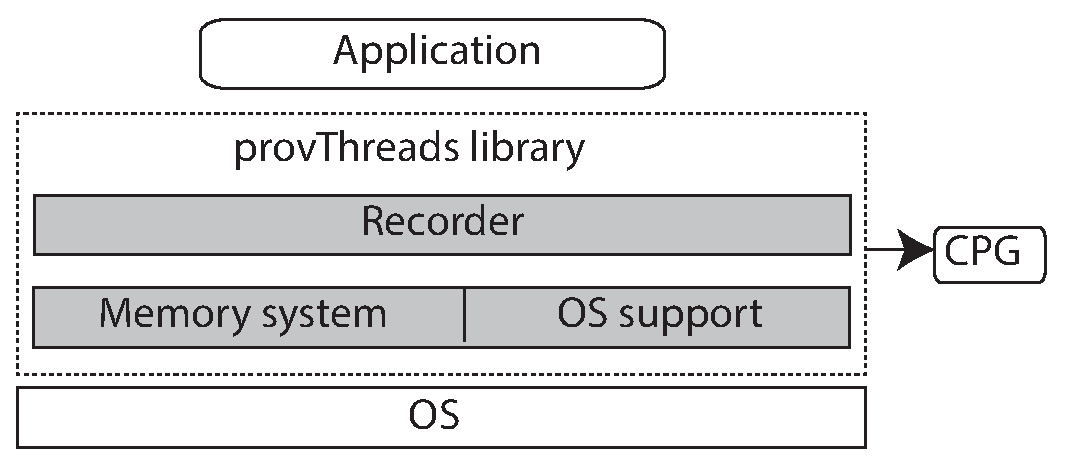
\includegraphics[scale=.4]{figure/System-basic-architecture}
  \caption{\projecttitle architecture. (System components are shown in grey boxes.)}
   
  \label{fig:basicSystem}

\end{figure}



\subsection{Memory System}


\myparagraph{Memory protection} A central challenge of the implementation of the algorithm is keeping track of the data dependencies for shared-memory accesses by all possible interleaving threads. Since monitoring every load and store to each memory word would be too costly, we instead rely on the OS's (hardware-assisted) page fault mechanism to keep track of reads and writes at the granularity of memory pages.

To derive the read and write sets during thunk execution,  \projecttitle~uses standard memory protection  mechanism and signal handlers. In particular, \projecttitle protects the address space using {\tt mprotect(PROT\_NONE)} at the beginning of each thunk. This forces a trap (and the corresponding OS signal) the first time a page is read or written to in a given thunk. The respective signal handler, which is implemented by the \projecttitle library, records the information about the access, and also resets the protection bits so that subsequent accesses to the same page by the same thread in the same thunk can proceed without generating a trap, and therefore avoid a
latency penalty.

However, a naive page protection mechanism raises an important problem because all threads in a process share the same virtual memory
structures (namely the TLB and page table entries with the respective protection bits). This makes it difficult to keep track of which
threads are responsible for which memory accesses or to enforce different protections for different threads. Otherwise, we need to re-protect the page after serving every load and store instruction causing a large number of page faults.
%(E.g., an access to a given memory location may or may not be the first access in a thunk depending on which thread is performing the access.)
To address this problem, \projecttitle implements threads as separate
processes (an idea originally proposed by Grace~\cite{grace-oopsla-2009} and also used in Dthreads~\cite{dthreads-sosp-2011}).

\myparagraph{Private address space} \projecttitle  implements threads as separate processes thus allowing each thread has its own private address space and control over the virtual
memory structures.   This gives us the ability to manipulate the page protection of threads individually while providing a simple way to implement the release consistency memory
model. In particular, \projecttitle uses the {\tt clone} system call to fork off a new process on {\tt pthread\_create()}. The process that implements the newly created thread (i.e., the child process) already
shares parts of the execution context with the parent process (which implements the calling thread) such as file descriptors and signal handlers.


But this raises a new problem, which is that, unlike threads, processes do not share their address spaces. We address this by taking advantage of the RC memory model we defined for \projecttitle, where threads share the updates only at synchronization points.  To implement the RC memory model, we use shared memory commit of Dthreads that allows threads to communicate at well-defined synchronization points.


\myparagraph{Shared memory commit} This shared memory commit is implemented using memory mapped files. In
particular, the virtual address ranges for the shared portions (globals and heap) of
the address space are mapped to memory mapped files, which are managed by the
\projecttitle library. These address ranges correspond to the heap and
the static (i.e., globals) regions.  During thread creation,
\projecttitle marks these address ranges as a private copy-on-write
mapping (using {\tt MAP\_PRIVATE} in {\tt mmap()}). The effect of this
is that whenever the child thread tries to write to a memory location,
the OS makes a thread-private copy of the memory page containing the
modification.  At synchronization points, the thread computes a {\em diff}
for each dirty page by performing a byte-level comparison between the
dirty page and the shared page. The deltas are then atomically
copied to the shared memory page; if there are overlapping writes
to the same memory location we resolve them using a last-writer wins policy.
\subsection{Recorder}

\subsection{OS Support}
\section{Evaluation}
\label{sec:evaluation}

In this section, we present an experimental evaluation of \projecttitle based on the implementation described in  \secref{implementation}. Our evaluation answers the following questions.

\begin{itemize}
\item What overheads does \projecttitle impose for recording data provenance? ($\S$~\ref{subsec:overheads})
\item How do these overheads scale with increases in the size of input data? ($\S$~\ref{subsec:data-size-overheads})
\item What are the sources for the provenance overheads? ($\S$~\ref{subsec:overheads-breakdown})
\end{itemize}



\subsection{Experimental Setup}
We first describe the experimental setup used for the evaluation.

\myparagraph{Experimental platform} We used an Intel Xeon processor based
multicore architecture as our host machine for our evaluation. The
host system consists of 8 cores (16 threads) of Intel(R) Xeon(R) CPU Processor D-1540
(12M Cache, 2.00 GHz) and 32 GB of DRAM main memory. The host
machine is running Linux with kernel 4.2.0 in 64-bit mode.


\myparagraph{Applications and dataset}  We evaluated \projecttitle with applications from two multithreaded benchmark suites: Phoenix 2.0 \cite{phoenix} and PARSEC 3.0 \cite{parsec}. Table~\ref{tab:apps} lists the applications used for the evaluation along with the input data and benchmark parameters.


\myparagraph{Measurements}  For all experiments,  we report time measurements, i.e., run-time comparison between the native {\tt pthreads} execution, and \projecttitle execution.  All applications were compiled using GCC 5.2.1 compiler with -$o3$ optimization flag. For all performance measurements, we report the average over 10 runs with minimum and maximum values discarded.



%\myparagraph{Metrics: Time and Work}  We consider two types of measures to report the performance metrics: {\em time} and {\em work}. In a nutshell, time measurements reflect the end user perceived latency, whereas work measurements assess the overall resource (CPU) utilization.  More specifically,  time refers to the end-to-end computation time for the multithreaded applications. Work refers to the total computation performed by all threads, and it is measured as the cumulative CPU time for all threads. To measure work, we used the CPU accounting controller in {\tt cgroups} to account the CPU usage of all threads.

%\myparagraph{Measurements} All applications were compiled using GCC 5.2.1 compiler with -$o3$ optimization flag. For all performance measurements, we report the average over 10 runs with minimum and maximum values discarded.


%\myparagraph{Additional results} Due to the space limitation, we only present  time measurements for all experiments. The work measurements are available online on the following anonymized link:  
% \href{http://www.mpi-sws.org/\~bhatotia/}{\tt http://www.mpi-sws.org/\textasciitilde bhatotia/}


%\if 0
%\begin{figure}[h]
%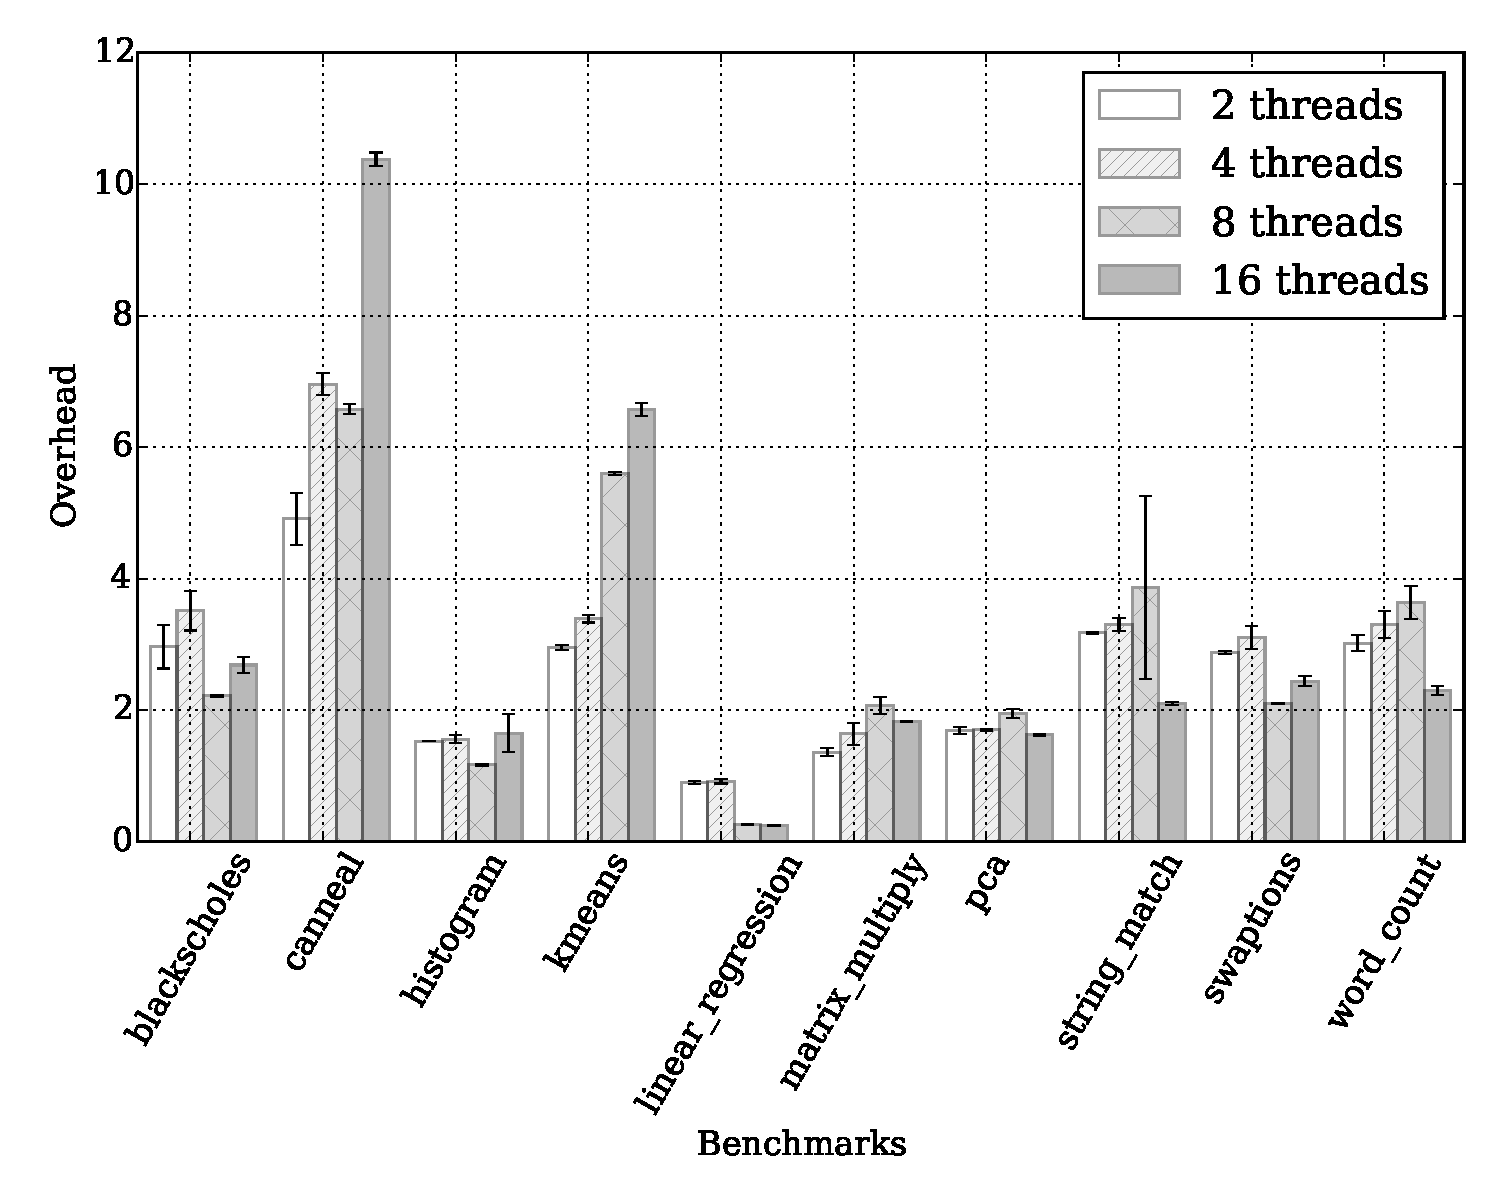
\includegraphics[width=8cm]{figure/benchmarks/times-inspector.pdf}
%\end{figure}
%
%\begin{figure}[h]
%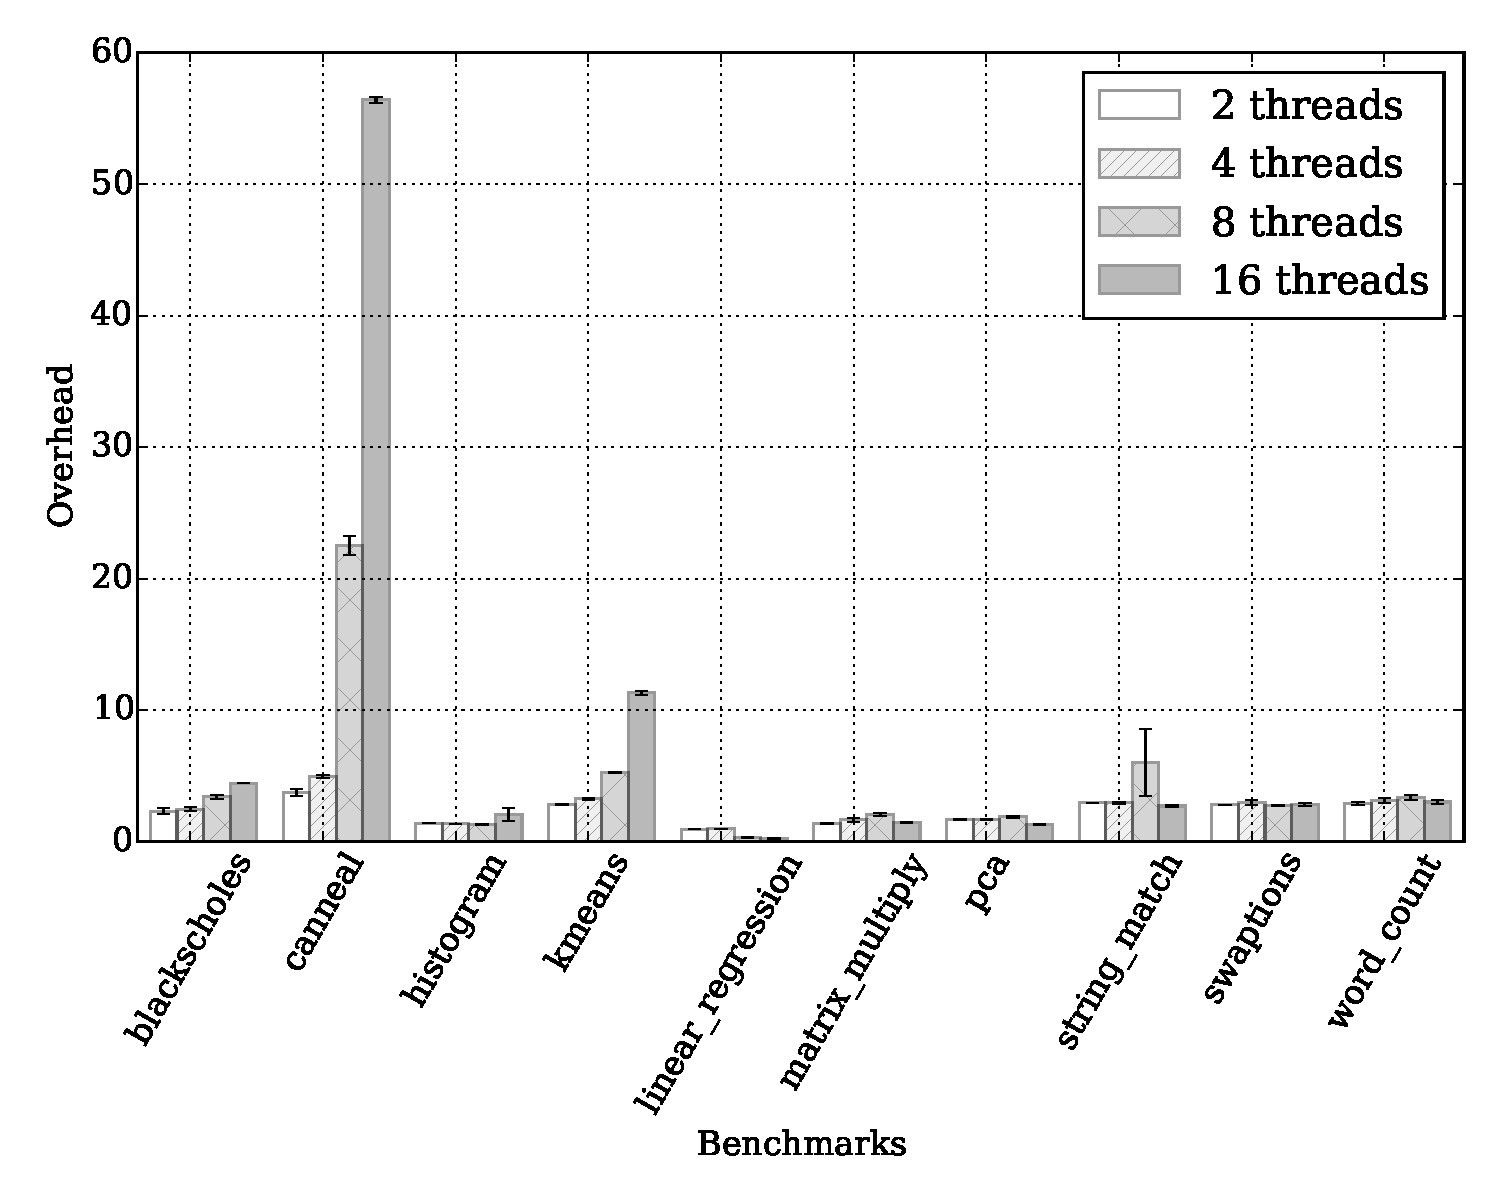
\includegraphics[width=8cm]{figure/benchmarks/cpu-cycles-inspector.pdf}
%\end{figure}
%
%\begin{figure}[h]
%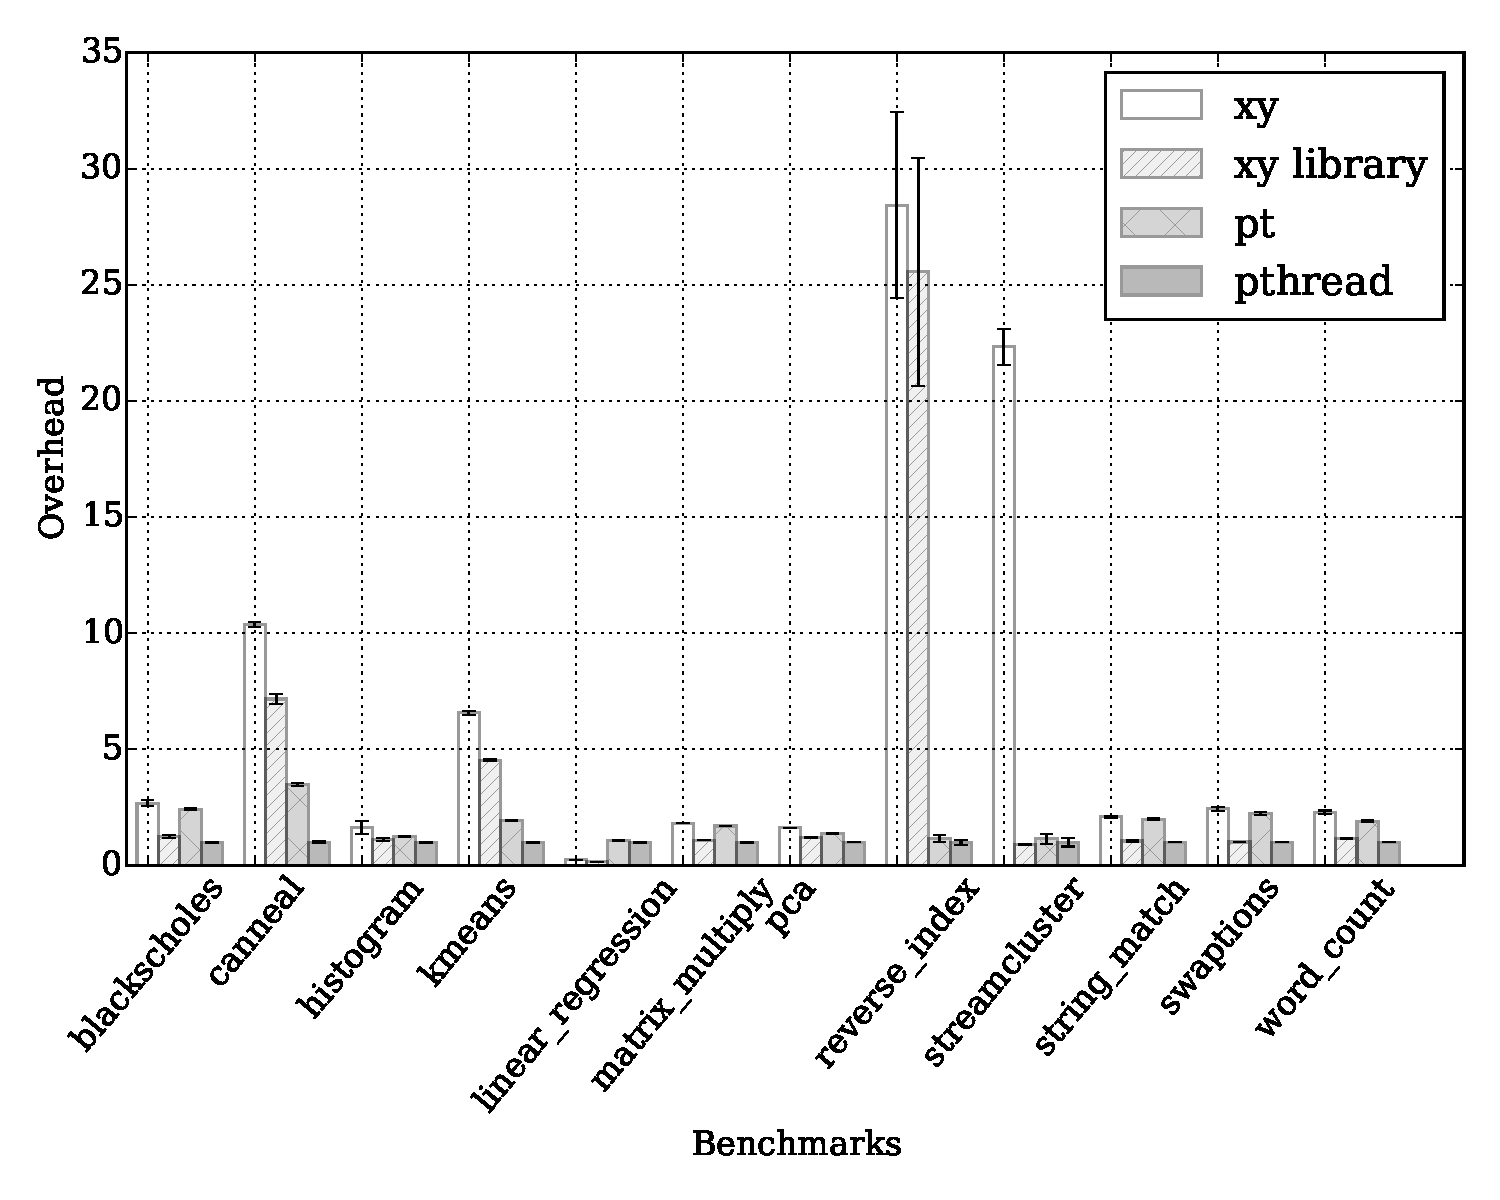
\includegraphics[width=8cm]{figure/benchmarks/times-16-threads.pdf}
%\end{figure}
%
%\begin{figure}[h]
%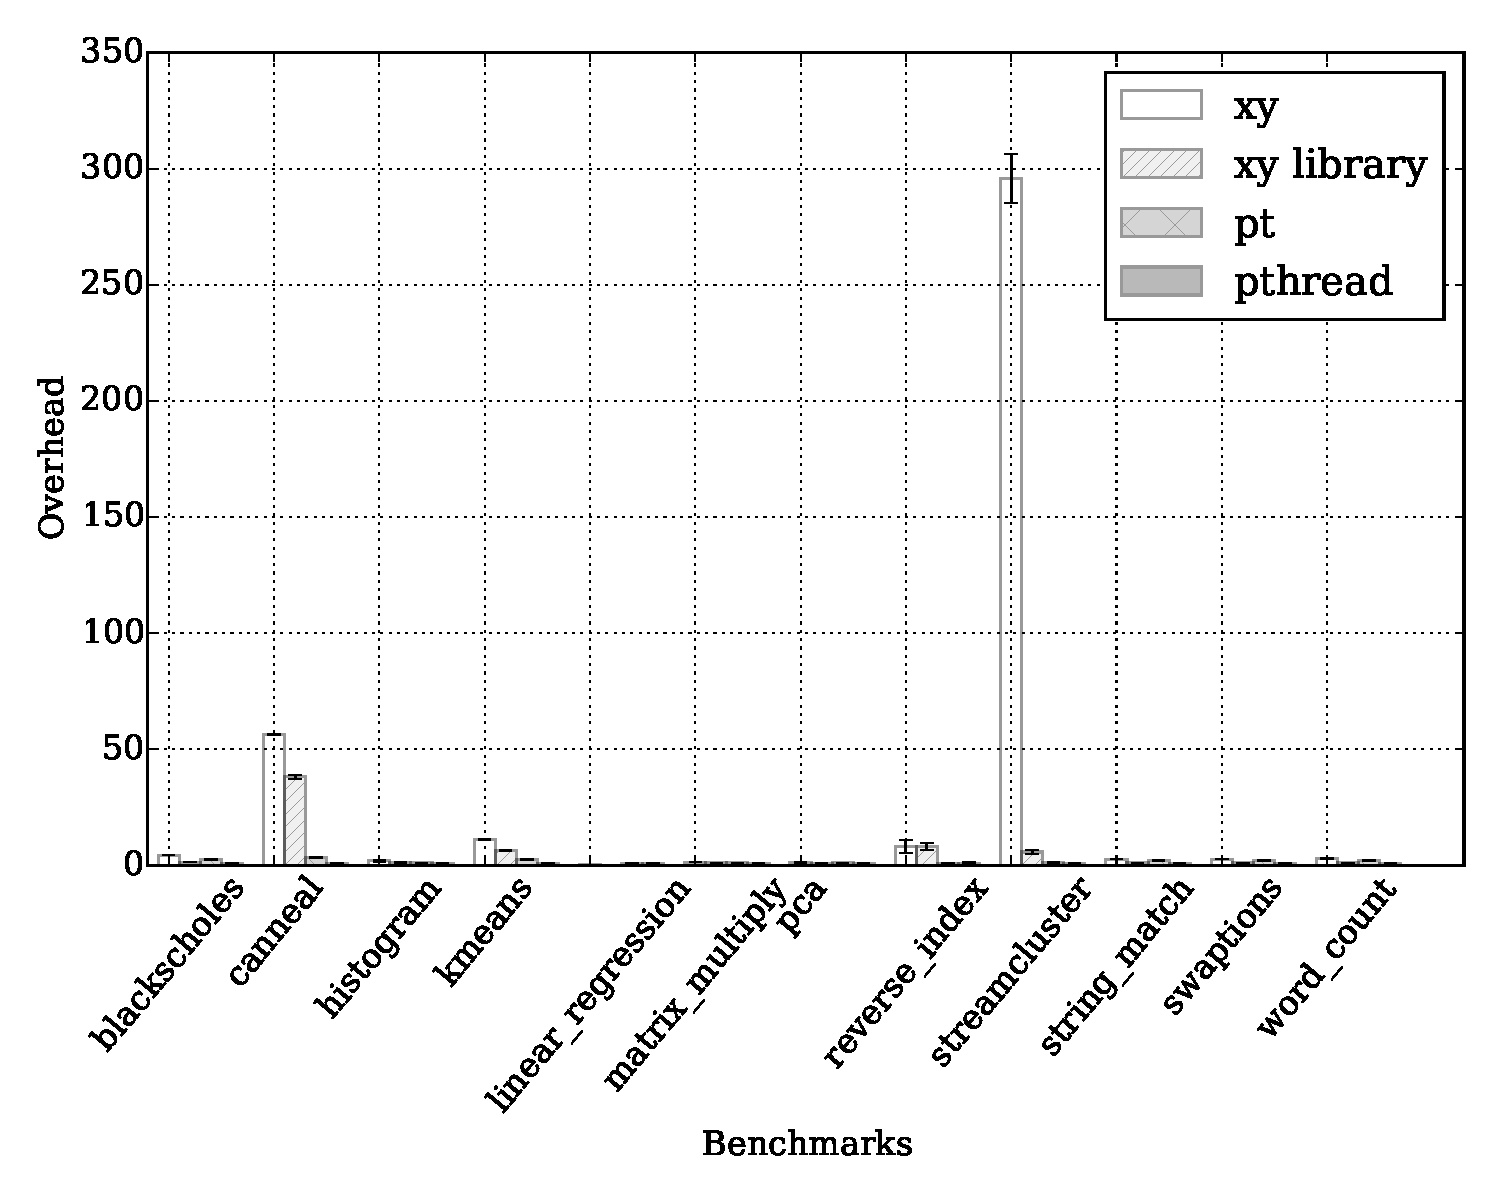
\includegraphics[width=8cm]{figure/benchmarks/cpu-cycles-16-threads.pdf}
%\end{figure}
%
%\begin{figure}[h]
%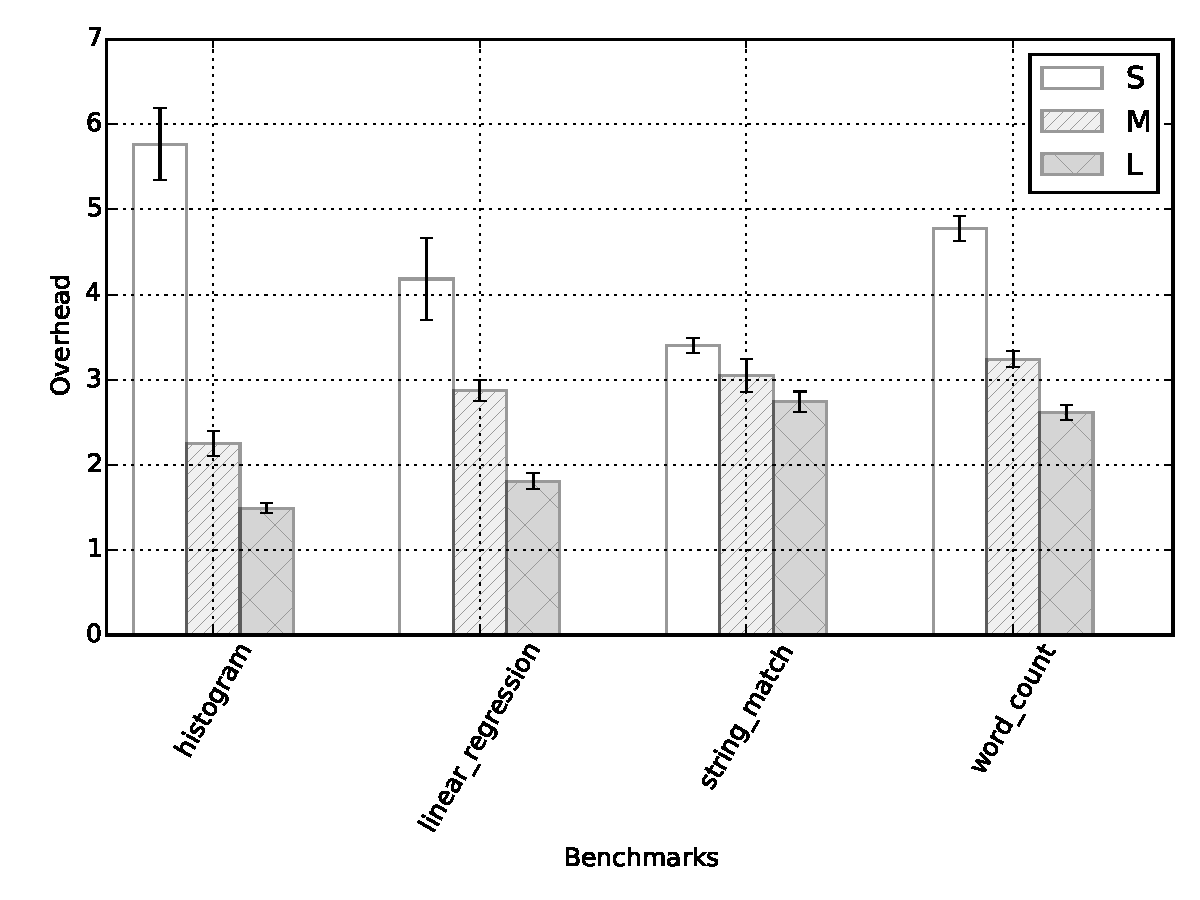
\includegraphics[width=8cm]{figure/benchmarks/worksize-times-inspector.pdf}
%\end{figure}
%\fi 
%
%\myparagraph{Performance metrics: Work and Time}  For each run, we consider two types of measures: \emph{work} and
% {\em time}. Work refers to the total amount of
%computation performed by all threads and is measured as the total
%run-time of all threads. Time refers to the amount of (end-to-end)
%run-time to complete the parallel computation. Both metrics are important
%and complementary: time measurements reflect the end user perceived latency,
%whereas work measurements assess the overall resource (CPU) utilization.

\subsection{Provenance Overheads}
\label{subsec:overheads}


\begin{figure}[t]
\centering
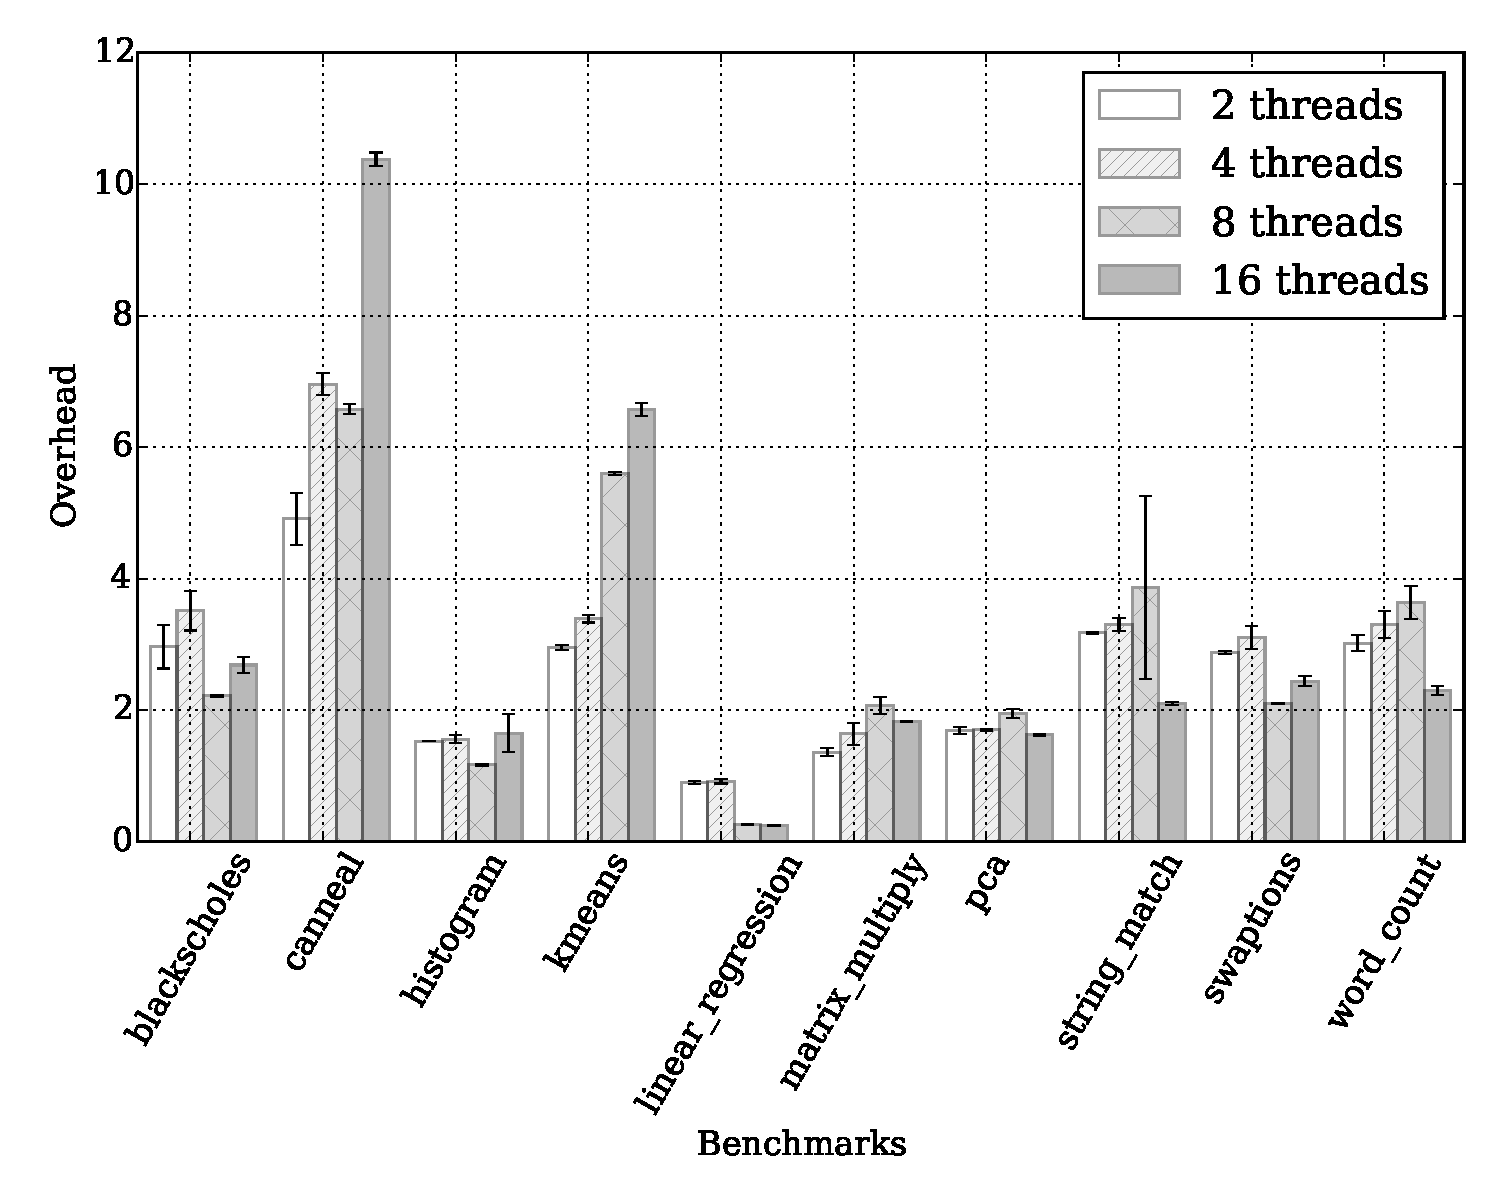
\includegraphics[scale=0.46]{figure/benchmarks/times-inspector.pdf}
\caption{Performance overhead  over native execution with increasing number of threads.}
\label{fig:overheads}
\end{figure}



\subsection{Scalability w.r.t. Input Data Sizes}
\label{subsec:data-sizes-overheads}




\begin{figure}[t]
\centering
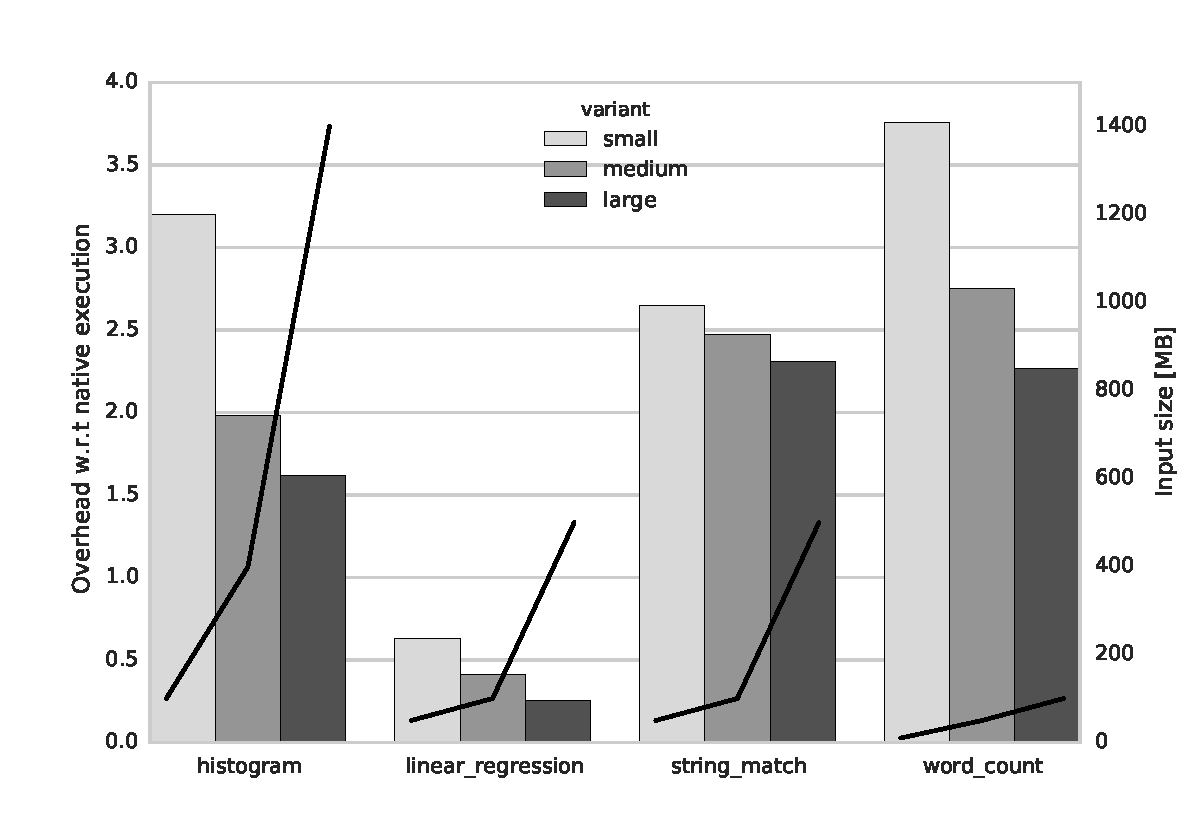
\includegraphics[scale=0.3]{figure/benchmarks/worksize-times-xy.pdf}
\caption{Scalability of overheads with increase in the input data sizes with $16$ threads. }
\label{fig:data-size-overheads}
\end{figure}






\subsection{Overheads Breakdown}
\label{subsec:overheads-breakdown}

\begin{figure}[t]
\centering
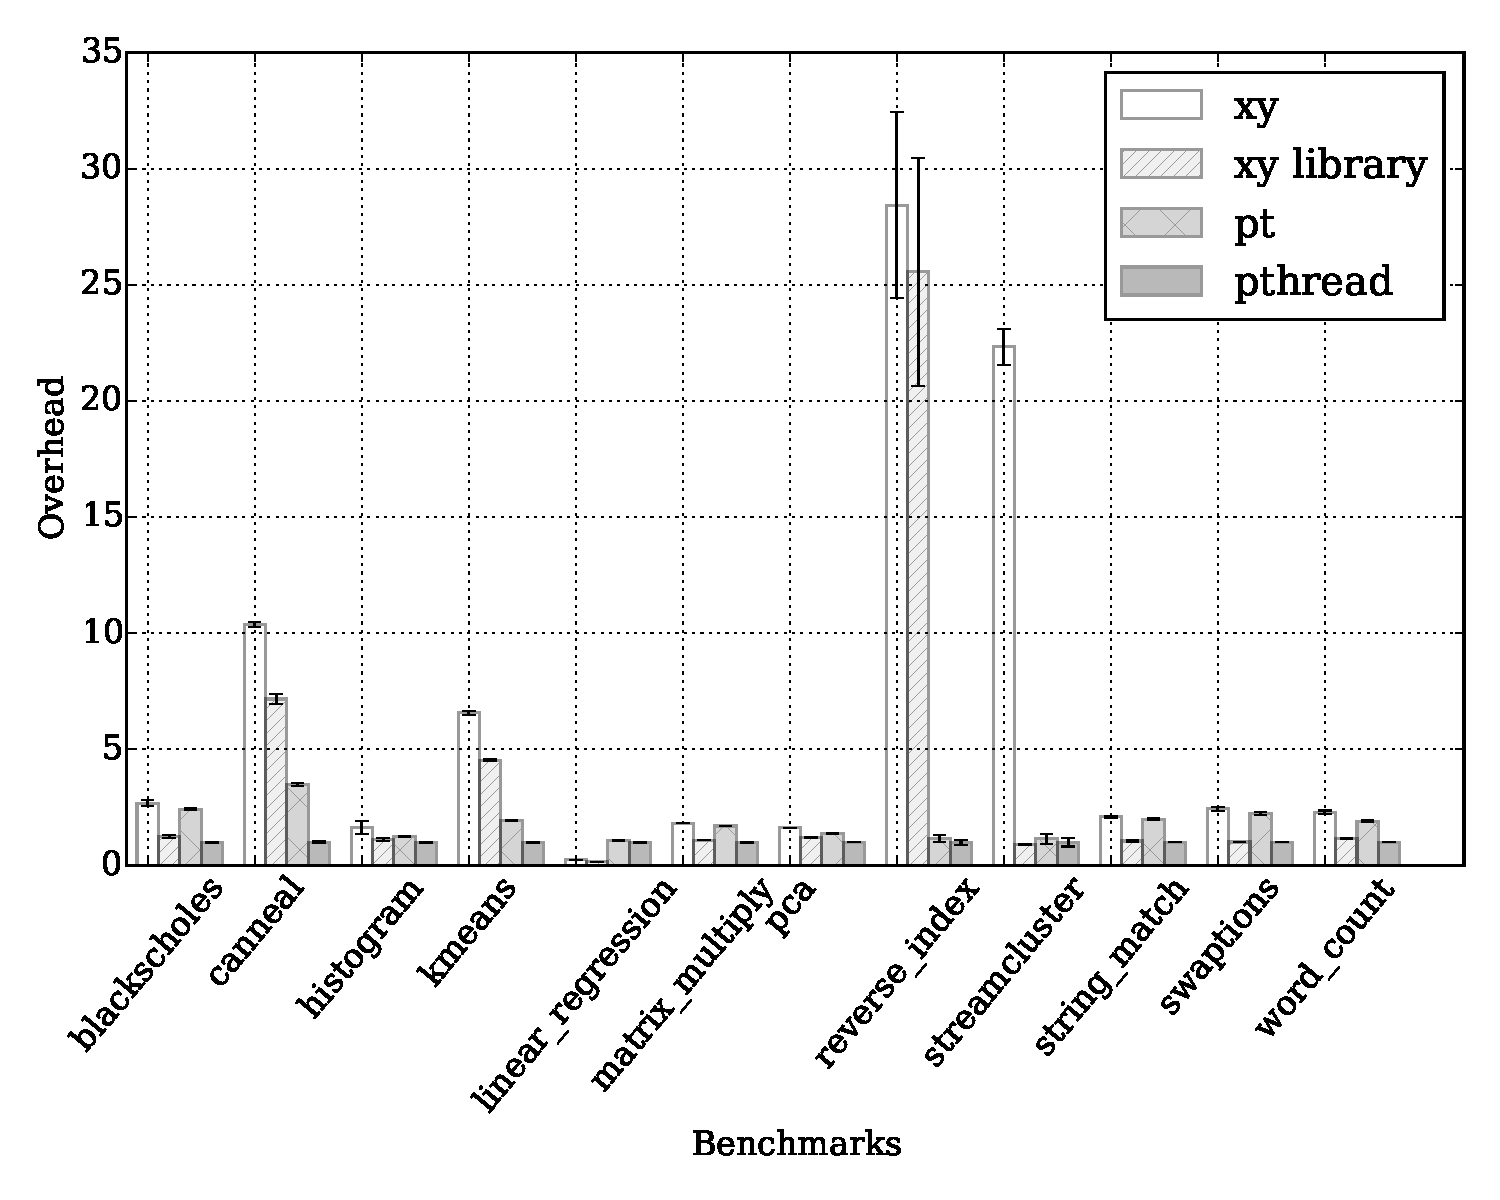
\includegraphics[scale=0.43]{figure/benchmarks/times-16-threads.pdf}
\caption{Performance overhead breakdown with $16$ threads --- except for streamcluster, where overhead for 15 threads is shown}
\label{fig:overheads-breakdown}
\end{figure}


% -*- root: ../main.tex -*-

% Dmitrii: couldn't find a way to make dynamic multicolumn with csvreader, so just copy-pasted result here from tables/data/avxbenches-stats.csv

\begin{table*}[t]
\footnotesize
\centering

\begin{tabular}{l | r r r || l | r r r}
%[-8pt]
\bfseries Bench & \bfseries ILP & \bfseries AVX & \bfseries inc & \bfseries Bench & \bfseries ILP & \bfseries AVX & \bfseries inc \\
\hline                    
\hline
hist      & 2.13  & 60.1  &  8.56 & black    & 1.77 & 76.6 & 1.70 \\
km        & 2.58  & 73.2  &  6.37 & dedup    & 1.75 & 60.7 & 4.64 \\
linreg    & 1.70  & 55.0  & 10.49 & ferret   & 1.81 & 67.2 & 4.32 \\
mmul      & 0.96  & 77.2  &  4.47 & fluid    & 1.54 & 75.8 & 2.43 \\
pca       & 2.28  & 77.4  &  6.82 & scluster & 1.22 & 77.1 & 3.77 \\
smatch    & 3.26  & 52.1  & 32.72 & swap     & 2.06 & 70.5 & 3.50 \\
wc        & 2.24  & 70.9  &  6.14 & x264     & 2.00 & 59.3 & 3.26 \\
\hline
\end{tabular}


\caption{Runtime statistics for versions of benchmarks with 16 threads: ILP (in instr/cycle), fraction of AVX instructions (in percents), and increase in number of all instructions w.r.t. native.}
\label{tab:apps}

\end{table*}






\section{Related Work}
\label{sec:related}

Data provenance is a well-studied concept because of it's wide applicability in different complex computer systems. In this section, we review some of the previous work in data provenance from different domains.





\myparagraph{Storage systems} Storage systems supporting provenance collect meta-data of newly created objects in the system (via the OS support), and  maintain their lineage information such as the chain of ownership and the transformations performed on objects. In this context, one of the most important line of work is on Provenance-Aware Storage Systems (PASS) that automates collection and maintenance of provenance~\cite{pass-papers, pass-atc} of objects in the system. In addition, PASS also supports queries, tracing the lineage of objects, upon the provenance data. In contrast to PASS that tracks objects in storage systems, our focus is on tracing the lineage of shared-memory accesses in multithreaded programs at the granularity of memory pages. Like PASS, we also rely on the OS support for tracking of memory pages.


\myparagraph{Database systems} Provenance has been shown to be important in databases to understand the lineage of annotations in materialized views,  to probabilistic databases, to data integration, curated databases, and many more applications (see a survey paper for more details~\cite{provenance-database-tutorial}). Almost, all existing provenance work in databases leverage explicit database schema and structured layout of input records in tables to build the provenance graph, whereas, \projecttitle does not assume any structured layout of the input data.


\myparagraph{``Big Data" analytics} Data provenance is being increasingly used in ``big data"  processing for  debugging complex workflows~\cite{nova, sixt, lipstick}, and also for incremental computation~\cite{incoop, slider, dryadinc, cbp}.  These ``big data" systems leverage the underlying data-parallel programming model such as MapReduce~\cite{mapreduce} or Dryad~\cite{dryad} for building the provenance graph. In particular, these systems construct the provenance graph based on the data-flow graph generated from the data-parallel programming model. The data-flow graph is represented by a DAG, where vertices are tasks (e.g. Map or Reduce), and directed edges correspond to data and control dependencies between tasks. Instead of relying on the underlying data-parallel programming model for building the provenance graph,  \projecttitle derives the graph automatically for the general shared-memory multithreaded programming model.



\myparagraph{Distributed and network systems} Many distributed and network systems propose provenance techniques for tracing the  execution of distributed protocols to provide accountability, fault detection, forensics, verifiability, network debugging, negative provenance~\cite{snp, exspan, wu-2014-negative-provenance, dtap}. These systems leverage the semantics of distributed protocols to derive a state-machine, and capture the lineage information by modifying the state-machine. To make the lineage secure in the presence of adversaries in distributed settings, they further embed techniques like tamper-proof logging~\cite{peer-review} along lineage for non-repudiability.   As opposed to these semantic-based approaches, again, we target general multithreaded programs, albeit at the granularity of memory pages instead of protocol-specific provenance.



\myparagraph{Multithreaded programs}



\myparagraph{Programming languages} Programming languages researchers develop language-based provenance approaches relying on a new language with special data-types. These language-based approaches derive the provenance graph using techniques such as  program slicing~\cite{roly} or advancement such as self-adjusting computation~\cite{Acar05, roly-calculas}. In contrast, our work supports unmodified existing programs without relying on any language-level support or a new type system.


\section{Conclusion}
\label{sec:conclusion}

In this paper, we presented \projecttitle, a data provenance library for multithreaded programs. Our approach targets existing executables, relies on OS-specific mechanisms and new ISA extensions of \intelpt  to efficiently build the {\em Concurrent Provenance Graph (CPG)}. The CPG records control, data, and schedule dependencies for the shared-memory multithreaded program execution. Our solution is straightforward to deploy: it simply replaces the {\tt pthreads} library, allowing existing applications to benefit from our approach with no re-compilation or code changes. \projecttitle's source code is publicly available for further use in a wide-range of workflows for data provenance. 


 
 %\vspace{-2mm}


\bibliographystyle{abbrv}

\bibliography{main}



\end{document}
